%%=============================================================================
%% Methodologie
%%=============================================================================

\chapter{\IfLanguageName{dutch}{Methodologie}{Methodology}}%
\label{ch:methodologie}

Het onderzoek werd uitgevoerd in een iteratieve cyclus, waarbij de verschillende fasen van het project elkaar opvolgden en elkaar beïnvloedden.
Deze sectie beschrijft in grote lijnen de verschillende fasen van het onderzoek, de doelstellingen en de gebruikte methodologieën.
Figuur~\ref{fig:methodologie} toont een flowchart van de methodologie, waarin de verschillende fasen en hun onderlinge relaties worden weergegeven.
De labels op de pijlen geven de belangrijkste deliverables van elke fase aan, die als input dienen voor de volgende fase(s).
\begin{figure}[H]
  \centering
  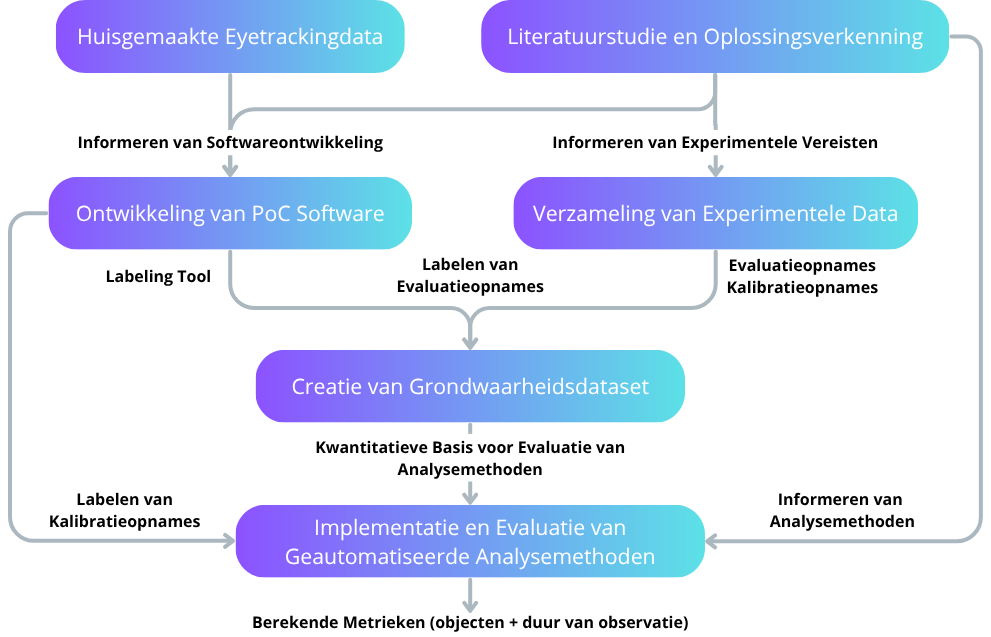
\includegraphics[width=0.9\textwidth]{methodologie.png}
  \caption{Flowchart van de methodologie van het onderzoek.}
  \label{fig:methodologie}
\end{figure}

\section{Literatuurstudie}

De literatuurstudie vormde een iteratief proces gedurende het gehele onderzoek, beginnend met een brede initiële verkenning en 
later verfijnd en aangevuld naarmate specifieke vragen tijdens het project opdoken. 
Het overkoepelende doel was een grondig en actueel inzicht te verwerven in de relevante domeinen. 
Hierbij lag de focus op de volgende gebieden: 
\begin{enumerate}
  \item Onderzoeken hoe de evaluatie van observatieprestaties momenteel wordt uitgevoerd, met bijzondere aandacht aan de nood aan een geautomatiseerde aanpak.
  \item De huidige stand van zaken in eyetracking-technologie, met aandacht voor hoofd-gemonteerde systemen zoals de Tobii Pro Glasses 3 en de analyse van de hieruit voortkomende data.
  \item State-of-the-art technieken binnen Computer Vision, waaronder objectdetectie (bv. YOLO, DETR, Grounding DINO), segmentatie (bv. Mask R-CNN, SAM, FastSAM) en image embedding (bv. CLIP, DINOv2).
  \item Bestaande integraties van eyetracking en Computer Vision.
\end{enumerate}
Wetenschappelijke publicaties, technische documentatie en relevante open-sour\-ce projecten werden hiervoor systematisch 
geraadpleegd en kritisch geanalyseerd.
Hoofdstuk~\ref{ch:stand-van-zaken} beschrijft uitvoerig de bevindingen van deze literatuurstudie.

\section{Oplossingsverkenning}

Voortbouwend op de inzichten uit de literatuurstudie, richtte de tweede fase zich op het verkennen en evalueren van verschillende 
conceptuele oplossingsstrategieën om de centrale onderzoeksvraag te beantwoorden. 
Het doel was om een reeks potentiële benaderingen te formuleren voor het automatisch analyseren 
van eyetrackingdata in combinatie met computervisiemodellen, en hieruit de meest veelbelovende te 
selecteren voor de ontwikkeling van de Proof-of-Concept (PoC). 
Dit proces omvatte het conceptueel ontwerpen van diverse pipelines, waarbij de inputs (eyetracking-opnames, objectdefinities) 
en de gewenste outputs (geobserveerde objecten, observatieduur) als leidraad dienden. 
De strategieën varieerden op vlak van algemene aanpak, de typen computervisiemodellen 
en de rol van de blikdata in het proces. 
Elke strategie werd kwalitatief beoordeeld op criteria zoals verwachte accuraatheid, complexiteit van implementatie, 
computationele vereisten en flexibiliteit. 
Deze analyse resulteerde in een beargumenteerde keuze voor de strategie die als basis diende voor het onderzoek, 
zoals gedetailleerd in Hoofdstuk~\ref{ch:oplossingsstrategieen}.

\section{Huisgemaakte Eyetrackingdata}

Voor het onderzoek en het uitwerken van de PoC software-applicatie, was het belangrijk om zicht te krijgen op de werking van de Eyetracker en de bijhorende software.
Daarom werd deze ontleend uit het Zorglab van HoGent voor een periode van 3 weken. 
Tijdens deze periode werden thuis verschillende opnames gemaakt in een woonkamer met diverse objecten, met de volgende specifieke doelstellingen:
\begin{itemize}
    \item Het leren werken met de Tobii Pro Glasses 3 en de bijhorende software.
    \item Nagaan hoe men de eyetrackingdata kan exporteren naar een bruikbaar formaat via de WiFi-verbinding van de eyetracker.
    \item Een dataset creëren die kan dienen als basis voor het uitwerken van de PoC.
\end{itemize}
Deze opnames werden niet gebruikt voor de uiteindelijke evaluatie van de PoC, aangezien de data afkomstig zijn van tests waarbij de onderzoeker zelf de eyetracker droeg.
Hierdoor is er sprake van mogelijke bias, wat de objectiviteit van de data in het gedrang brengt.

\section{Proof of Concept Software Applicatie}

Een kernonderdeel van deze bachelorproef was de ontwikkeling van een Proof-of-Concept (PoC) softwareapplicatie. 
Het hoofddoel van deze fase was het ontwerpen en implementeren van een werkend prototype dat de beoogde workflow ondersteunt: van het importeren van ruwe eyetracking-opnames tot het genereren van gelabelde data die als basis kan dienen voor analyse. 
De methodologie omvatte de selectie van een passende, moderne technologie-stack (o.a. Python, FastAPI, HTMX, SQLite) gericht op modulariteit en toekomstige uitbreidbaarheid. 
Een significant onderdeel was het ontwerp en de implementatie van een semi-automatische labeling-tool, bedoeld om de efficiëntie van het labelingsproces te verhogen. 
Er werd ingezet op duurzame software-ontwikkelpraktijken zoals type hinting en containerisatie (Docker) om de mogelijkheid tot onderhoud en reproduceerbaarheid te waarborgen. 
De resulterende applicatie, inclusief de architectuur, componenten en technische keuzes, wordt uitvoerig beschreven in Hoofdstuk~\ref{ch:ontwikkeling}.

\section{Experimenteel Onderzoek}

Zoals eerder vermeld, werd de thuisopgenomen dataset niet gebruikt voor de evaluatie van de PoC. 
Om een onbevooroordeelde dataset te verkrijgen en om de modaliteiten van de uitwerking te valideren (bijvoorbeeld: invloed van de afstand tussen de Eyetracker en het object, en de aard van de objecten), werd er een gecontroleerd experiment opgezet in het Zorglab van HoGent.
Het doel van dit experiment was om een dataset te creëren die als grond-waarheid diende voor de metrieken die de PoC berekent (bekeken objecten en tijdsduur).
Op de campus werden studenten van diverse opleidingen gevraagd om deel te nemen aan het experiment.
De 14 resulterende opnames werden daarna gelabeld via de labeling-tool van de PoC, met een manuele kwaliteitscontrole om de betrouwbaarheid van de data te waarborgen.
Voor een uitgebreide beschrijving van het opzet en de uitvoering van het experiment, inclusief de gebruikte methodologieën, wordt verwezen naar Hoofdstuk~\ref{ch:experiment}.

\section{Creatie van een Grondwaarheidsdataset}

Om de prestaties van de geautomatiseerde analysemethoden objectief te kunnen evalueren, was de creatie van een nauwkeurige 
grondwaarheidsdataset noodzakelijk. Het doel van deze fase was om, voor elke evaluatieopname uit het experiment, 
frame-per-frame vast te stellen welke van de 15 gedefinieerde objecten daadwerkelijk door de deelnemer werden bekeken. 
De methodologie startte met het voorbereiden van de ruwe opnamedata (video en blikdata). 
Vervolgens werden de evaluatieopnames gelabeld met behulp van de ontwikkelde labeling-tool (zie Hoofdstuk~\ref{ch:ontwikkeling}).
Hierbij segmenteerde de onderzoeker objecten waar de blik van de deelnemer op rustte, met behulp van het SAM2-model en de trackingfunctionaliteit van de labeling-tool.
Deze initiële segmentaties werden daarna gefilterd op basis van de geregistreerde blikpunten, waarbij een cirkelvormig kijkgebied moest overlappen met het segmentatiemasker. 
Dit resulteerde in een dataset die per frame de bekeken objecten, hun bounding boxes en maskeroppervlakte specificeert. 
De correctheid werd manueel gevalideerd. De gedetailleerde stappen van dit proces zijn beschreven in Hoofdstuk~\ref{ch:grondwaarheid}.

\section{Analyse van Observatieprestaties}

De laatste fase van het onderzoek focuste op het implementeren en evalueren van een geautomatiseerde analysepipeline om observatieprestaties te meten, 
conform de gekozen oplossingsstrategie (Strategie 4 uit Hoofdstuk~\ref{ch:oplossingsstrategieen}). 
Het doel was om automatisch te bepalen welke kritische objecten werden waargenomen en hoe lang, en dit te vergelijken met de grondwaarheidsdataset. 
De methodologie omvatte:
\begin{enumerate}
  \item Het toepassen van ``everything-segmentation'' en tracking met FastSAM op de evaluatieopnames.
  \item Het filteren van de resulterende segmenten op basis van objectgrootte en de geregistreerde 
  blikdata (overlap met het blikpunt), wat resulteerde in de te classificeren object ROIs (Regions of Interest).
  \item Het classificeren van deze ROIs met drie verschillende methoden: 
  \begin{itemize}
    \item Een DINOv2 image embedding model, dat de ROIs omzet naar vectorrepresentaties en deze vergelijkt met een Faiss vector-index van de kalibratieopnames.
    \item Een YOLOv11-classificatiemodel, dat specifiek getraind is op de objecten uit de kalibratieopnames.
    \item Het toepassen van een YOLOv11-objectdetectiemodel, dat de ROIs detecteert en de voorspellingen combineert met de eerdere FastSAM-segmen\-taties.
  \end{itemize}
\end{enumerate}
De prestaties van deze geautomatiseerde analysepipeline werden kwantitatief beoordeeld aan de hand van precisie, 
recall en F1-score ten opzichte van de grondwaarheidsdataset. 
De evaluatie ging echter verder dan deze kernmetrieken. 
Er werd een systematische hyperparameteroptimalisatie via een grid search uitgevoerd en modellen 
getraind met verschillende hoeveelheden data werden vergeleken. 
Bovendien vond een diepgaande analyse plaats van de aard van vals-positieve en vals-negatieve detecties, 
waarbij ook de invloed van factoren zoals objectgrootte werd onderzocht. 
Dit proces, inclusief de gedetailleerde methodologie en resultaten, wordt uitvoerig beschreven in Hoofdstuk~\ref{ch:analyse}.